\section{Main result: selective spectral learning at matched fit}
\label{sec:theorem}

We state the mechanism in the simplest serial model that has both cues,
a shared encoder, and a replicated contextual readout. Training inputs are
two sites: the pixel's own spectral coordinate $S$ and a contextual
coordinate $C$, both equal to the label. The encoder $W=(a,v)$ reads each
site with one coefficient; the head adds the spectral coordinate directly
and the contextual one through $M$ replicated readouts. Replication is the
only way width enters. The statement combines the serial instance, its
general-initialization corollary and the readout-normalization proposition
of Appendix~\ref{app:proofs}.

\begin{theorem}[Selective spectral learning at matched fit]\label{thm:serial}
Let $Y$ be uniform on $\{-1,1\}$, $x_1=(S,0)$, $x_2=(0,C)$,
and $S=C=Y$ in training. The shared encoder $W=(a,v)$ produces
$z_1=aS,z_2=vC$; the head is $F=z_1+bz_2$, $b=\sum_{j=1}^M\beta_j$.
For integer $M\ge1$, train $(W,\beta)$ by unit Euclidean gradient flow
on $\mathcal L=\mathbb E\log(1+e^{-YF})$, without other optimizer terms,
from fixed $a_0\in\mathbb R$, $v_0\ne0$, $\sum_j\beta_{j0}=0$.
Fix $m>0$ and $T_m=\inf\{t\ge0:q_J(t)\ge m\}$, $q_J=a+bv$;
thus $T_m=0$ if $a_0\ge m$.

\textbf{(a) Suppression.} If $a_0<m$, set $\Delta=m-a_0$,
$u_M=a(T_m)-a_0$. Then $T_m<\infty$ and
\[
 0<\frac{u_M}{\Delta}\le\frac1{1+Mv_0^2},
 \qquad Mu_M\longrightarrow\frac{\Delta}{v_0^2}\quad(M\to\infty).
\]
The spectral-only head $F=aS$ requires update $\Delta$.
If $q_F$ instead trains only $\beta$ from the same initialization with
$W$ frozen, then $q_J\ge q_F$ on $[0,T_m]$ and
$\sup_{0\le t\le T_m}(q_J-q_F)\le C_0/(p_0Mv_0^2)$,
where $C_0=1+2\Delta^2/v_0^2$ and $p_0=(1+e^{-a_0})^{-1}$.

\textbf{(b) Reversal.} On $S=Y,C=-Y$, the stopped margin is
$2a(T_m)-m$ when $a_0<m$, and $a_0$ otherwise.
Error is one if $a_0<m/2$ and $Mv_0^2>m/(m-2a_0)$;
it is zero for $a_0\ge m/2$. The spectral-only comparator has zero
error for every $a_0$.
For $(a_0,v_0)\sim\mathcal N(0,\sigma^2I_2)$, $\sigma>0$, with
zero-sum readouts and the same stopping rule,
$\lim_{M\to\infty}\mathbb E_{W_0}\mathrm{Err}_{\rm rev}
=\Phi(m/(2\sigma))$, where $\Phi$ is the standard normal CDF.

\textbf{(c) Normalization.} Replace $b$ by
$M^{-1/2}\sum_j\gamma_j$, with $\sum_j\gamma_{j0}=0$ and the same
$(a_0,v_0)$ and unit rates. The aggregate $(a,v,b)$ dynamics equal
those at $M=1$ for every width.
\end{theorem}
\begin{remark}[Special initialization]
For $(a_0,v_0)=(0,1)$, the scalar-logit GGN blocks
$G_{\thetap\thetap},G_{\phip\phip}$, $\thetap=(a,v)$,
$\phip=\beta$, give $\mathcal D_{\rm curv}(0)=M$
(generally $Mv_0^2$), and
$\Psi(m)/(M+1+2m^2)\le T_m\le\Psi(m)/(M+1)$,
where $\Psi(m)=m+e^m-1$.
\end{remark}

\paragraph{Proof sketch.}
Dividing the flow by $\dot a=\varrho>0$, $\varrho=(1+e^{q_J})^{-1}$,
gives $dv/da=b$ and $db/da=Mv$, hence with $u=a-a_0$
\[
 v=v_0\cosh(\sqrt M u),\qquad
 b=\sqrt M v_0\sinh(\sqrt M u),\qquad
 q_J=a_0+u+\tfrac{\sqrt M v_0^2}{2}\sinh(2\sqrt M u),
\]
the balance invariant of gradient flow \citep{astra_du2018balance}. The
fitting equation $q_J(u_M)=m$ is strictly increasing in $u$ and
$\sinh x\ge x$ gives the update bound and its limit; a transformed-margin
comparison with the frozen path gives the finite-horizon gap. The sign of
the reversed margin $2a(T_m)-m$ and dominated convergence give (b). For
(c), differentiating the aggregate readout gives $\dot b=v\varrho$,
independent of $M$. Full proofs are in Appendix~\ref{app:proofs}.

\paragraph{What the theorem says, and what it does not.}
Replication acts as an effective learning rate on the contextual readout.
At the matched margin the spectral coefficient has moved by at most a
fraction $1/(1+Mv_0^2)$ of the update the spectral-only model needs; the
coefficient itself can be informative at initialization and remain so. It
is the \emph{adaptation} that is suppressed. When the initial spectral
coefficient is below half the margin and the width is large enough,
$Mv_0^2>m/(m-2a_0)$, the fitted joint model relies on context strongly
enough that contextual reversal misclassifies every example, while a
spectral-only comparator trained to its own hitting time of the same
margin is correct; at small $Mv_0^2$ the fitted model can be correct even
with $a_0<m/2$, so the failure is a finite-width statement, not a
universal one. The spectral-only comparator is trained to
its own hitting time; the frozen comparator is evaluated at the joint
path's elapsed times through $T_m$. Part (c) removes the width dependence
only: the normalized system is the $M=1$ system, which for
$(a_0,v_0)=(0,1)$ still fails under reversal for every $m>0$. Finally,
training each contextual readout at rate $\kappa$ instead of unit rate
gives $\dot b=\kappa Mv\varrho$ and the bound $1/(1+\kappa Mv_0^2)$: the
relative training speed of the contextual pathway, not width as such, is
the competition parameter the experiments manipulate.

\paragraph{Numerical check.}
The closed forms agree with a full $(2+M)$-parameter integration over
$525$ initialization--width--margin cases to a relative discrepancy of
$1.3\times10^{-11}$ in the endpoint quantities, with no bound violated, and
the Gaussian sweep approaches its limit $\Phi(1)$ ($0.8207$, $0.8380$,
$0.8397$ at $M=64$, $1024$, $16384$; Appendix~\ref{app:verification}). This
checks the algebra, not the claim beyond the model.

\begin{figure}[t]
\centering
\IfFileExists{figures/fig2_mechanism.pdf}{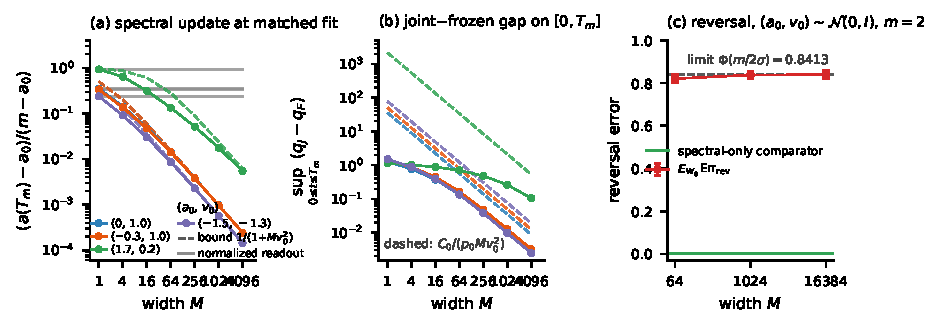
\includegraphics[width=0.92\linewidth]{figures/fig2_mechanism.pdf}}{\fbox{\rule{0pt}{2.1in}\rule{0.97\linewidth}{0pt}}}
\caption{The exact mechanism (Theorem~\ref{thm:serial}; $m=2.9$ unless
stated). (a) Spectral update fraction $u_M/\Delta$ at the matched margin
against width $M$ for four initializations $(a_0,v_0)$ (solid) with the
bound $1/(1+Mv_0^2)$ (dashed) and the normalized readout of part (c)
(grey, flat at the $M=1$ value). (b) Joint-minus-frozen margin gap
$\sup_{0\le t\le T_m}(q_J-q_F)$ with the bound $C_0/(p_0Mv_0^2)$ (dashed).
(c) Expected reversal error over $(a_0,v_0)\sim\mathcal N(0,I_2)$ against
$M$ for $m=2$, with the limit $\Phi(m/2)$; the spectral-only comparator has
error zero.}
\label{fig:mechanism}
\end{figure}
